\documentclass[a4paper,12pt]{article}

\usepackage{geometry}
\usepackage{amsmath}
\usepackage{amssymb}
\usepackage{graphicx}
\usepackage{booktabs}
\usepackage{float}
\usepackage{caption}
\usepackage{subcaption}
\usepackage[section]{placeins}
\usepackage{hyperref}
\usepackage{enumitem}
\usepackage{array}
\usepackage{tabularx}
\usepackage{indentfirst}
\usepackage{fancyhdr}

\geometry{left=2.5cm,right=2.5cm,top=2.55cm,bottom=2.55cm}
\hypersetup{colorlinks=true,linkcolor=black,citecolor=black,urlcolor=blue}
\captionsetup{font=small,labelsep=quad}
\setlist{itemsep=0.30em,topsep=0.55em}
\linespread{1.20}
\setlength{\emergencystretch}{3em}
\setlength{\parindent}{2em}
\setlength{\headheight}{15pt}
\setlength{\parskip}{0.15em}
\setlength{\textfloatsep}{0.75em plus 0.2em minus 0.15em}
\setlength{\floatsep}{0.65em plus 0.2em minus 0.15em}
\setlength{\intextsep}{0.65em plus 0.2em minus 0.15em}
\renewcommand{\topfraction}{0.9}
\renewcommand{\bottomfraction}{0.85}
\renewcommand{\textfraction}{0.08}
\renewcommand{\floatpagefraction}{0.75}
\raggedbottom

\pagestyle{fancy}
\fancyhf{}
\fancyhead[C]{LLM-Assisted Long-Horizon Prediction of High-Dimensional Chaotic Systems}
\fancyfoot[C]{\thepage}

\newcommand{\xvec}{\mathbf{x}}
\newcommand{\dt}{\Delta t}
\newcommand{\crmse}{\mathrm{CRMSE}}
\newcommand{\mse}{\mathrm{MSE}}

\title{\textbf{LLM-Assisted Long-Horizon Predictive Modeling of High-Dimensional Chaotic Systems}\\
\large A Case Study on Lorenz-63 and Lorenz-96}
\author{Xingtao Zhong\textsuperscript{*} \quad Yuxuan Huang\textsuperscript{*} \quad Zhiqi Hao\\
\textsuperscript{*}Co-first authors / equal contribution\\
Student IDs: 25120617 \quad 25120619 \quad 25120621\\
Course: Introduction to Artificial Intelligence}
\date{\today}

\begin{document}

\maketitle
\thispagestyle{empty}

\begin{abstract}
This paper studies long-horizon multi-step prediction for chaotic dynamical systems. With the assistance of large language models, we first use the Lorenz-63 system to show that ordinary supervised learning models can fit short-term state transitions but fail to maintain stable recursive rollout. We then construct a 10-dimensional Lorenz-96 dataset and compare several models, including Baseline LSTM, PINN LSTM, Transformer, Hybrid LSTM, and Ultimate Hybrid. The main evaluation metric is the final cumulative RMSE over a 500-step rollout. The results show that one-step accuracy alone does not guarantee long-term stability. The proposed Ultimate Hybrid model, which combines an imperfect RK4 physical solver, Transformer-based residual learning, PINN loss, and refined scheduled sampling, achieves the lowest final cumulative RMSE of 12.80. The study suggests that, for high-dimensional chaotic prediction, machine learning is more effective as a residual corrector for physical models than as a fully black-box replacement.
\end{abstract}

\noindent\textbf{Keywords:} large language model; Lorenz-96; high-dimensional chaotic system; long-horizon prediction; recursive rollout; Transformer; PINN; hybrid correction

\newpage
\tableofcontents
\newpage

\section{Introduction}

The main difficulty of chaotic-system prediction is not only the one-step prediction error, but also the amplification of small errors during long recursive rollout. For deterministic nonlinear systems such as the Lorenz family, a tiny deviation in the initial or predicted state may lead to a rapidly diverging trajectory. Therefore, a low one-step RMSE on a test set does not necessarily mean that the model can stably predict hundreds of future steps.

This paper focuses on the following question: how can we design a predictive model that combines physical structure, sequence memory, and long-horizon stability for high-dimensional chaotic systems? We first use the Lorenz-63 system as an intuitive baseline case. Its three-dimensional structure makes it suitable for demonstrating that short-term local state transitions are learnable, while long-horizon recursive rollout remains difficult. The central task of this paper is then extended to the 10-dimensional Lorenz-96 system, whose higher dimensionality and periodic coupling make long-term prediction more challenging.

The main contributions of this work are:
\begin{enumerate}
    \item We use Lorenz-63 to verify the phenomenon that short-term prediction is learnable but long-term rollout is limited by chaotic error amplification.
    \item We build a recursive rollout evaluation framework for the Lorenz-96 system and use cumulative RMSE as the primary metric.
    \item We compare Residual LSTM, PINN LSTM, Transformer, Hybrid LSTM, and Ultimate Hybrid models under the same long-horizon setting.
    \item We propose an Ultimate Hybrid architecture that combines an imperfect physical solver, Transformer residual learning, PINN constraints, and refined scheduled sampling.
    \item We analyze the contribution and limitation of each component based on reproducible CSV outputs and generated figures.
\end{enumerate}

\section{Dataset Construction and Exploratory Analysis}

\subsection{Data Source and Feature Description}

The data used in this project are generated by numerical integration of dynamical-system equations rather than downloaded from a static external dataset. The Lorenz-63 part contains three state variables, $x$, $y$, and $z$, and forms a short-term supervised-learning task such as predicting $x(t+k\dt)$. The Lorenz-96 part contains $N=10$ coupled state variables, $x_1,\dots,x_{10}$, and the main task is to predict the next full state vector from a historical window.

From a machine-learning perspective, each sample corresponds to either a single time slice or a historical time window. The input features describe the current position and local evolution trend in phase space, while the target variable describes the next state or state increment. All experimental data are generated by Python scripts and saved in \texttt{results/*.csv}, making the workflow reproducible and traceable.

\subsection{Correlation Heatmap}

Figure \ref{fig:corr_heatmap_en} shows the correlation heatmap for the Lorenz-63 supervised-learning dataset. The heatmap indicates that neighboring states and future targets are statistically related, which explains why short-term local prediction is feasible. However, such local correlation does not imply long-term predictability, because recursive rollout repeatedly feeds small model errors back into the system.

\begin{figure}[htbp]
\centering
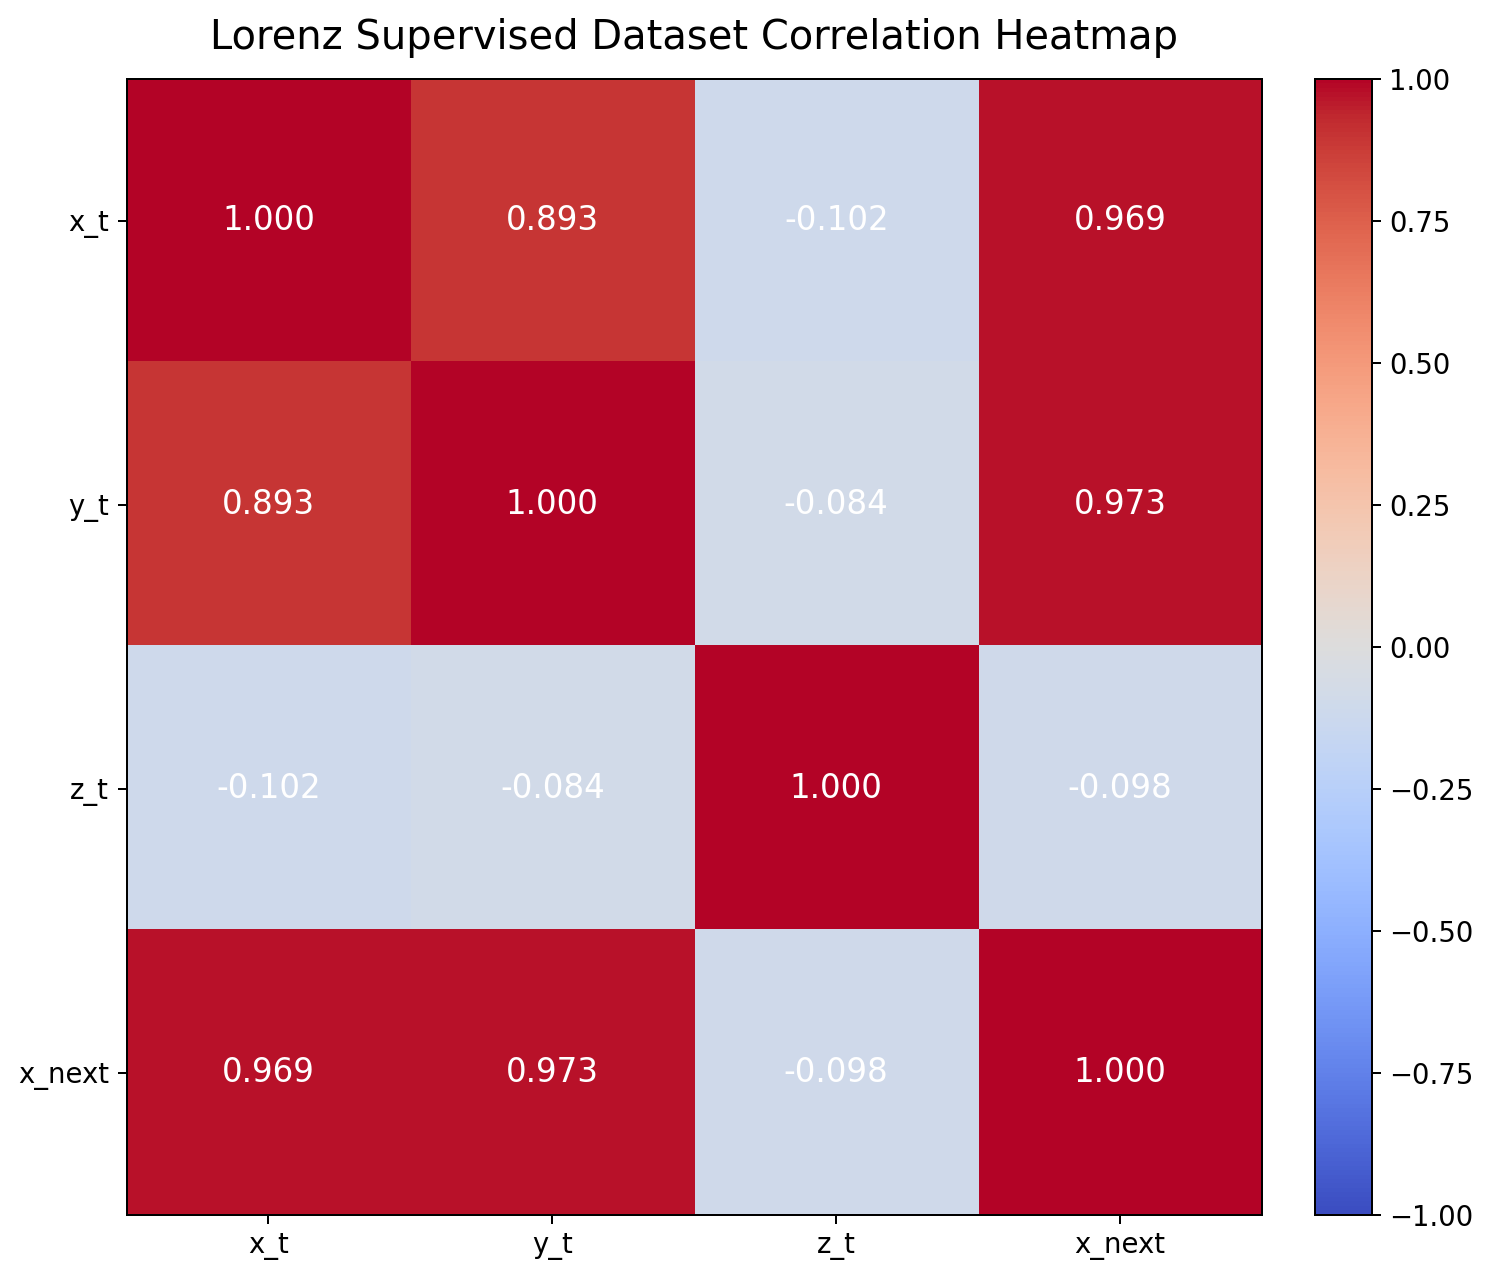
\includegraphics[width=0.70\textwidth]{figures/correlation_heatmap_en.png}
\caption{Correlation heatmap of the Lorenz-63 supervised-learning dataset. The heatmap checks linear feature relations and supports the claim that short-term local states are learnable.}
\label{fig:corr_heatmap_en}
\end{figure}

\subsection{Preprocessing}

The preprocessing pipeline includes missing-value checking, chronological train-test splitting, and standardization. Since the data are generated by numerical integration, no missing values are expected, but the output files are still checked. The train and test sets are split by time order instead of random shuffling to avoid future information leakage.

For models based on gradient descent, including MLP, LSTM, and Transformer, \texttt{StandardScaler} is used to place different variables on comparable scales. This improves optimization stability and prevents dimensions with larger numerical ranges from dominating the loss. Tree-based models do not strictly require standardization, but a unified preprocessing pipeline makes the experimental procedure easier to verify.

\section{Lorenz-63: Short-Term Learnability and Long-Term Limitation}

\subsection{Lorenz-63 Equation and Experimental Purpose}

The classical Lorenz-63 system is defined by three coupled ordinary differential equations:
\begin{align}
\frac{dx}{dt} &= \sigma(y-x),\\
\frac{dy}{dt} &= x(\rho-z)-y,\\
\frac{dz}{dt} &= xy-\beta z.
\end{align}
We use the standard parameter setting
\begin{equation}
\sigma=10,\quad \rho=28,\quad \beta=\frac{8}{3}.
\end{equation}
The trajectory is generated using \texttt{scipy.integrate.solve\_ivp}, with initial state $(1,1,1)$, simulation interval $[0,50]$, and 10000 sampled points. Figure \ref{fig:lorenz_attractor_en} shows the generated Lorenz attractor.

\begin{figure}[htbp]
\centering
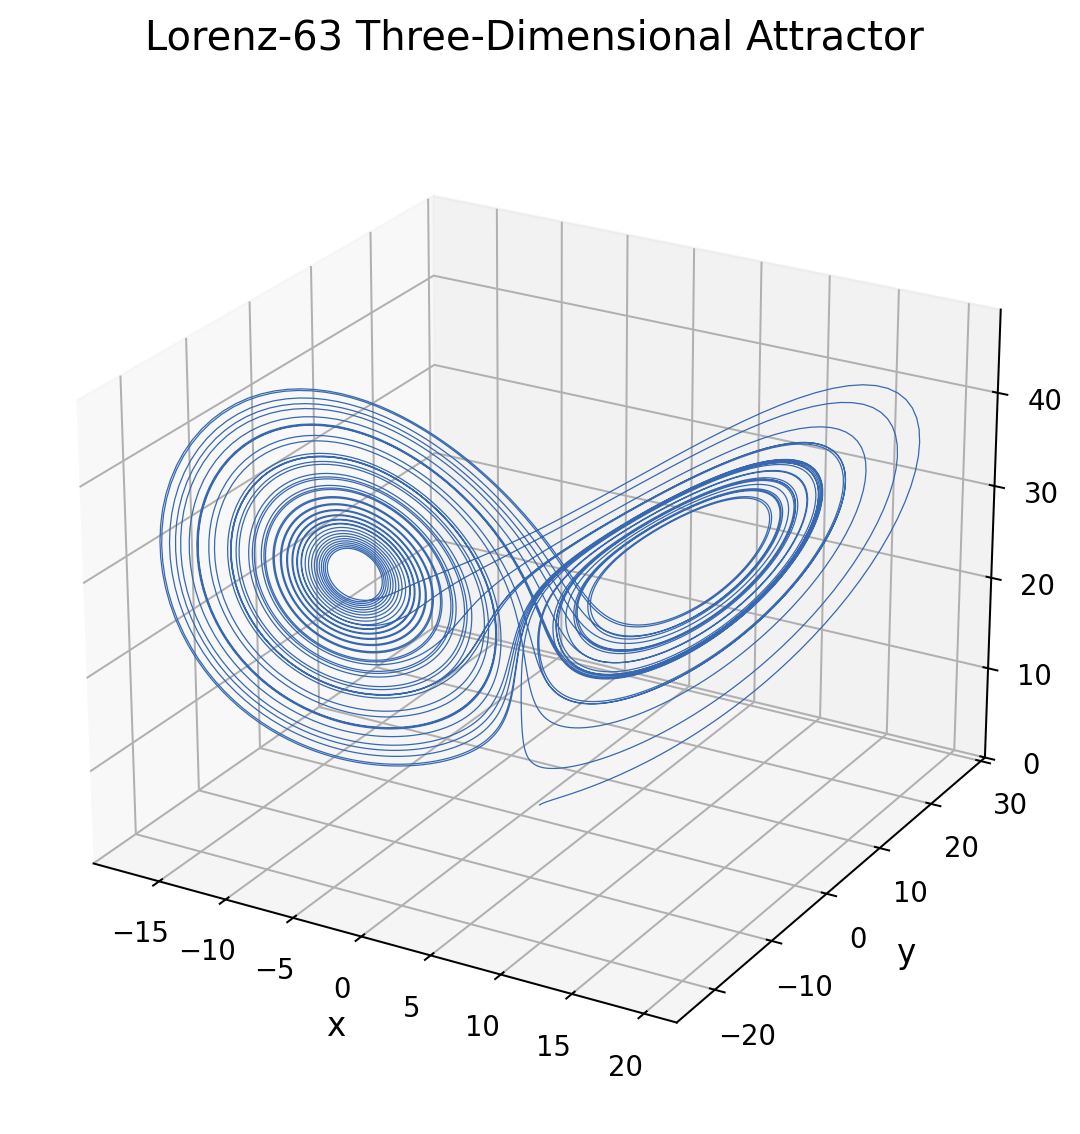
\includegraphics[width=0.68\textwidth]{figures/lorenz_attractor_en.png}
\caption{Three-dimensional Lorenz-63 attractor. This system is used to illustrate short-term fitting and long-term divergence in chaotic prediction.}
\label{fig:lorenz_attractor_en}
\end{figure}

\subsection{Short-Term Prediction and Rollout Divergence}

Table \ref{tab:lorenz63_short_en} reports the test-set results for the original short-term task, predicting $x(t+10\dt)$. Random Forest and MLP clearly outperform Linear Regression, showing that local nonlinear mappings can be learned by supervised models.

\begin{table}[htbp]
\centering
\caption{Short-term single-variable prediction results for Lorenz-63. Data source: \texttt{results/model\_metrics.csv}.}
\label{tab:lorenz63_short_en}
\begin{tabular}{lccc}
\toprule
Model & RMSE & MAE & $R^2$ \\
\midrule
Linear Regression & 0.5457 & 0.4437 & 0.9952 \\
Random Forest & 0.0805 & 0.0507 & 0.9999 \\
MLP & 0.0757 & 0.0599 & 0.9999 \\
\bottomrule
\end{tabular}
\end{table}

However, when the prediction horizon is expanded to $k=500$, the state RMSE rises to 10.9789 for Random Forest and 14.0980 for MLP. In a stricter 500-step recursive rollout setting, the model only receives the true state at the initial time and then repeatedly uses its own prediction as input. The final cumulative RMSE is shown in Table \ref{tab:lorenz63_rollout_en}.

\begin{table}[htbp]
\centering
\caption{500-step recursive rollout results for Lorenz-63 baseline models. Data source: \texttt{results/rollout\_results.csv}.}
\label{tab:lorenz63_rollout_en}
\begin{tabular}{lc}
\toprule
Model & Final Cumulative State RMSE \\
\midrule
Linear Regression & 20.2244 \\
Random Forest & 14.5356 \\
MLP & 19.8142 \\
\bottomrule
\end{tabular}
\end{table}

\begin{figure}[htbp]
\centering
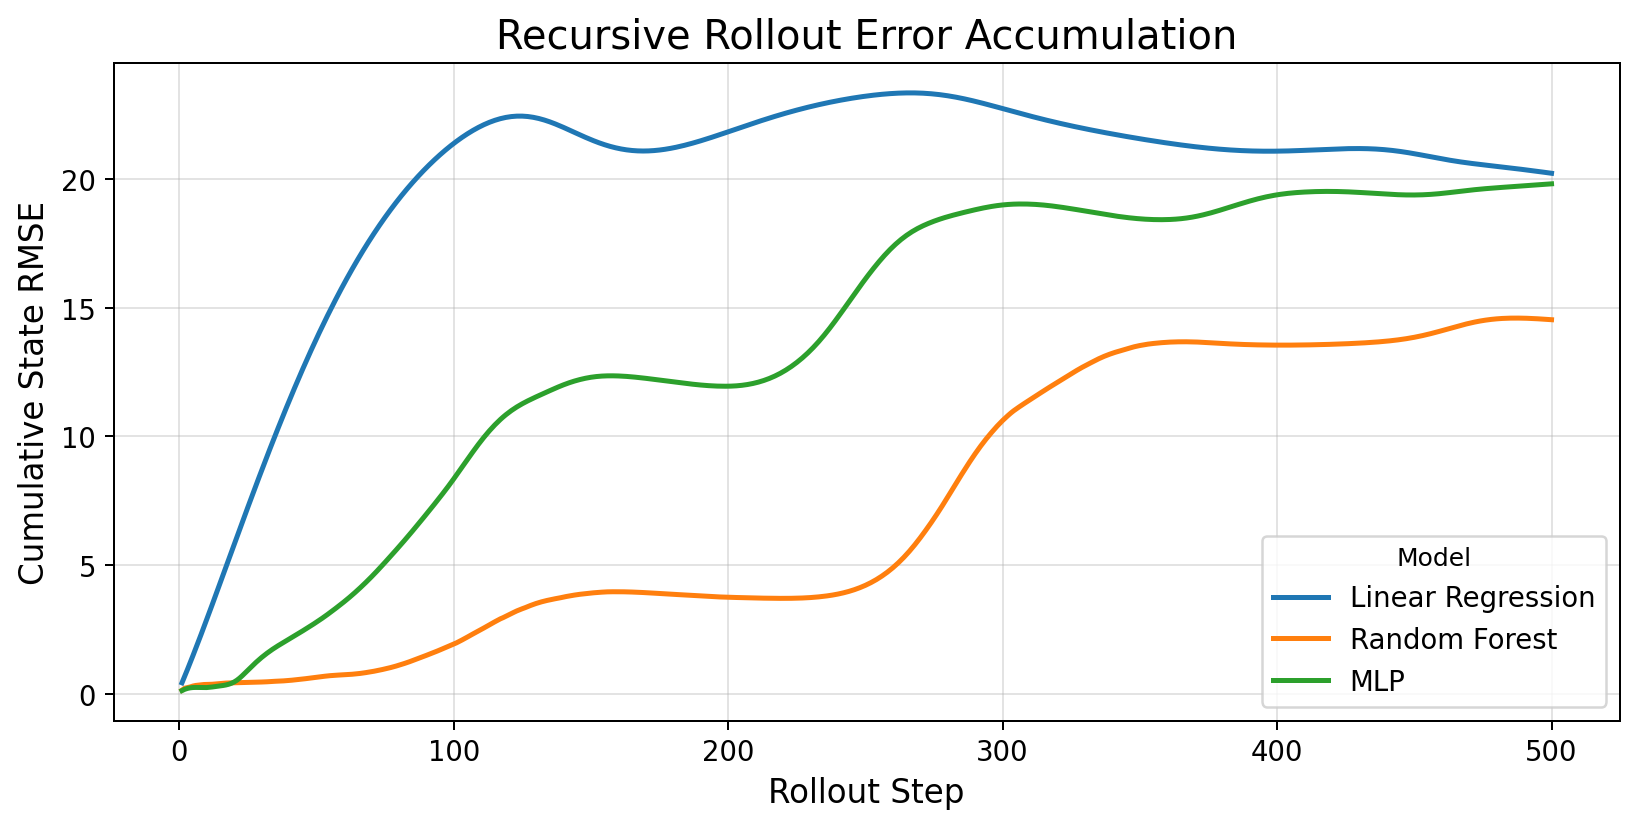
\includegraphics[width=0.78\textwidth]{figures/rollout_error_en.png}
\caption{Cumulative error of Lorenz-63 baseline models during recursive rollout. Short-term errors are repeatedly fed into the next step and gradually become long-term trajectory deviations.}
\label{fig:lorenz63_rollout_en}
\end{figure}

This result motivates the Lorenz-96 experiments: the real challenge is not one-step fitting, but long-horizon stability.

\section{Lorenz-96 and Multi-Step Prediction Definition}

\subsection{Lorenz-96 Dynamics}

Lorenz-96 is a common benchmark system for high-dimensional chaotic prediction. This paper uses the $N=10$ dimensional system:
\begin{equation}
\frac{dx_i}{dt}=(x_{i+1}-x_{i-2})x_{i-1}-x_i+F,\quad i=1,\dots,N.
\end{equation}
Periodic boundary conditions are applied:
\begin{equation}
x_{i+N}=x_i.
\end{equation}
The true forcing parameter is set to
\begin{equation}
F_{\mathrm{true}}=8.0,
\end{equation}
which places the system in a chaotic regime. The simulation interval is $[0,100]$, with 10000 sampled points. The initial state is a small perturbation around $F$:
\begin{equation}
\xvec_0=(F+0.01,F,\dots,F).
\end{equation}
Training and test sets are split chronologically into the first 80\% and last 20\%.

\subsection{Window-Based Sequence Prediction}

For Lorenz-96, the model input is a historical window of length $w$:
\begin{equation}
\mathbf{X}_t=(\xvec_{t-w+1},\xvec_{t-w+2},\dots,\xvec_t)\in \mathbb{R}^{w\times N}.
\end{equation}
The one-step prediction task is
\begin{equation}
\hat{\xvec}_{t+1}=f_\theta(\mathbf{X}_t).
\end{equation}
During evaluation, recursive rollout is used:
\begin{align}
\hat{\xvec}_{t+1} &= f_\theta(\xvec_{t-w+1},\dots,\xvec_t),\\
\hat{\xvec}_{t+2} &= f_\theta(\xvec_{t-w+2},\dots,\xvec_t,\hat{\xvec}_{t+1}),\\
&\ \vdots \notag\\
\hat{\xvec}_{t+m} &= f_\theta(\hat{\xvec}_{t+m-w},\dots,\hat{\xvec}_{t+m-1}).
\end{align}
This evaluation setting is closer to real long-term prediction and more clearly exposes stability problems.

\subsection{Cumulative RMSE}

We use the final cumulative RMSE over a 500-step rollout:
\begin{equation}
\crmse(T)=
\sqrt{
\frac{1}{T}\sum_{m=1}^{T}
\left\|\xvec_{t+m}-\hat{\xvec}_{t+m}\right\|_2^2
}.
\end{equation}
Compared with one-step RMSE, $\crmse(T)$ reflects both per-step error and error accumulation under recursive input. All main Lorenz-96 results use $T=500$.

\section{Model Design: From Baseline LSTM to Ultimate Hybrid}

\subsection{Baseline LSTM and State-Increment Learning}

The natural baseline for sequence prediction is LSTM. Direct state prediction can be written as
\begin{equation}
\hat{\xvec}_{t+1}=f_{\theta}^{\mathrm{LSTM}}(\mathbf{X}_t).
\end{equation}
However, for continuous dynamical systems, the change between adjacent time steps is often easier to learn than the absolute state. Therefore, the LSTM is converted into a residual form:
\begin{align}
\Delta \hat{\xvec}_{t+1} &= g_{\theta}^{\mathrm{LSTM}}(\mathbf{X}_t),\\
\hat{\xvec}_{t+1} &= \xvec_t+\Delta \hat{\xvec}_{t+1}.
\end{align}
This design makes the model closer to a local numerical integrator.

\subsection{Scheduled Sampling}

In one-step training, the model always sees a true historical window. In rollout, it gradually sees its own predicted states. This difference is known as exposure bias or train-test mismatch. Scheduled sampling reduces the mismatch by using model predictions with increasing probability during multi-step training.

Let $p_e$ denote the teacher-forcing probability at epoch $e$. A simple linear decay is
\begin{equation}
p_e=\max\left(0,1-\frac{e}{0.8E}\right),
\end{equation}
where $E$ is the total number of epochs. In the Ultimate Hybrid model, a smoother inverse-sigmoid schedule is used:
\begin{equation}
p_e=\frac{k}{k+\exp(e/(E/10))}.
\end{equation}
The model is unrolled for $M=5$ steps during training:
\begin{equation}
\mathcal{L}_{multi}=\frac{1}{M}\sum_{m=1}^{M}\mse(\hat{\xvec}_{t+m},\xvec_{t+m}).
\end{equation}

\subsection{PINN Physical Constraint}

Pure data-driven models may produce updates that violate the underlying dynamics. We introduce a physics-informed neural network (PINN) loss \cite{raissi2019}. The Lorenz-96 vector field is denoted as
\begin{equation}
\mathbf{f}_{L96}(\xvec;F_{\mathrm{true}}).
\end{equation}
The finite-difference derivative implied by the model prediction is
\begin{equation}
\frac{\hat{\xvec}_{t+1}-\xvec_t}{\dt}.
\end{equation}
The physical loss is defined as
\begin{equation}
\mathcal{L}_{phys}=
\left\|
\frac{\hat{\xvec}_{t+1}-\xvec_t}{\dt}
-
\mathbf{f}_{L96}(\xvec_t;F_{\mathrm{true}})
\right\|_2^2.
\end{equation}
The total loss is
\begin{equation}
\mathcal{L}=\mathcal{L}_{data}+\lambda \mathcal{L}_{phys},
\end{equation}
with $\lambda=0.1$ in the implementation.

\subsection{Transformer for Historical Windows}

LSTM compresses historical information into recurrent hidden states, while Transformer uses self-attention to directly model relations among time steps \cite{vaswani2017}. The Transformer model embeds each 10-dimensional state into a 64-dimensional space, adds positional encoding, and processes the sequence using a two-layer Transformer encoder:
\begin{align}
\mathbf{Z}_t &= \mathrm{PE}(\mathrm{Linear}(\mathbf{X}_t)),\\
\mathbf{H}_t &= \mathrm{TransformerEncoder}(\mathbf{Z}_t),\\
\Delta\hat{\xvec}_{t+1} &= W\mathbf{H}_{t,-1}+b.
\end{align}
This structure allows the model to use local oscillations and short-term evolution trends inside the historical window.

\subsection{Imperfect Physical Solver and Residual Correction}

In many scientific problems, an approximate physical model is available. We simulate this situation by constructing an imperfect Lorenz-96 solver:
\begin{equation}
F_{\mathrm{imp}}=8.5,\qquad F_{\mathrm{true}}=8.0.
\end{equation}
Let $\Phi_{\dt}^{F_{\mathrm{imp}}}$ denote a one-step RK4 solver using $F_{\mathrm{imp}}$:
\begin{equation}
\xvec^{phys}_{t+1}=\Phi_{\dt}^{F_{\mathrm{imp}}}(\xvec_t).
\end{equation}
The hybrid model predicts the residual of this imperfect physical prediction:
\begin{align}
\Delta \hat{\xvec}^{res}_{t+1} &= g_\theta(\mathbf{X}_t),\\
\hat{\xvec}_{t+1} &= \xvec^{phys}_{t+1}+\Delta \hat{\xvec}^{res}_{t+1}.
\end{align}
Thus, the physical solver provides the main evolution direction, while the neural network only corrects systematic bias and approximation error.

\subsection{Ultimate Hybrid Architecture}

The Ultimate Hybrid model combines four components:
\begin{enumerate}
    \item an imperfect RK4 physical solver with $F_{\mathrm{imp}}=8.5$;
    \item a Transformer residual model that extracts features from historical windows;
    \item a PINN loss that constrains the predicted update direction;
    \item refined scheduled sampling with 5-step unrolled training.
\end{enumerate}
Mathematically, its one-step prediction is
\begin{equation}
\hat{\xvec}_{t+1}
=
\Phi_{\dt}^{F_{\mathrm{imp}}}(\xvec_t)
+
g_{\theta}^{\mathrm{Transformer}}(\xvec_{t-w+1},\dots,\xvec_t).
\end{equation}
The training objective is
\begin{equation}
\mathcal{L}_{UH}
=
\frac{1}{M}\sum_{m=1}^{M}
\left[
\mse(\hat{\xvec}_{t+m},\xvec_{t+m})
+
\lambda
\left\|
\frac{\hat{\xvec}_{t+m}-\tilde{\xvec}_{t+m-1}}{\dt}
-
\mathbf{f}_{L96}(\tilde{\xvec}_{t+m-1};F_{\mathrm{true}})
\right\|_2^2
\right],
\end{equation}
where $\tilde{\xvec}_{t+m-1}$ denotes the input state after scheduled sampling.

\section{Results and Analysis}

\subsection{Stage-Wise LSTM Optimization}

Table \ref{tab:lstm_phase_en} summarizes representative results from the Lorenz-96 LSTM optimization process. Baseline LSTM achieves a reasonable one-step score but still accumulates significant long-term error. Residual learning, LayerNorm, and gradient clipping improve Phase 1. However, the simple scheduled-sampling version in Phase 2 improves one-step RMSE but worsens 500-step rollout RMSE. This shows that multi-step training must be carefully designed for chaotic systems.

\begin{table}[htbp]
\centering
\caption{Stage-wise Lorenz-96 LSTM optimization results.}
\label{tab:lstm_phase_en}
\small
\begin{tabularx}{\textwidth}{@{}>{\raggedright\arraybackslash}Xccc@{}}
\toprule
Model Stage & One-step RMSE & One-step $R^2$ & Final 500-step RMSE \\
\midrule
Baseline LSTM & 0.7360 & 0.9531 & 13.9662 \\
Phase 1: residual + LayerNorm + clipping & 0.0417 & 0.9999 & 13.1749 \\
Phase 2: multi-step loss + scheduled sampling & 0.0356 & 0.9999 & 14.1880 \\
\bottomrule
\end{tabularx}
\end{table}

\subsection{Window-Length Ablation}

The historical window length $w$ determines how much past information is visible to the model. Too short a window may miss useful phase-space information, while too long a window may introduce redundant chaotic noise. Table \ref{tab:window_ablation_en} and Figure \ref{fig:window_ablation_en} show the ablation results.

\begin{table}[htbp]
\centering
\caption{Lorenz-96 LSTM window-length ablation. Data source: \texttt{results/lstm\_phase3\_summary.csv}.}
\label{tab:window_ablation_en}
\begin{tabular}{cc}
\toprule
Window Length $w$ & Final 500-step RMSE \\
\midrule
10 & 15.7545 \\
20 & 16.5752 \\
50 & 111.0108 \\
\bottomrule
\end{tabular}
\end{table}

\begin{figure}[htbp]
\centering
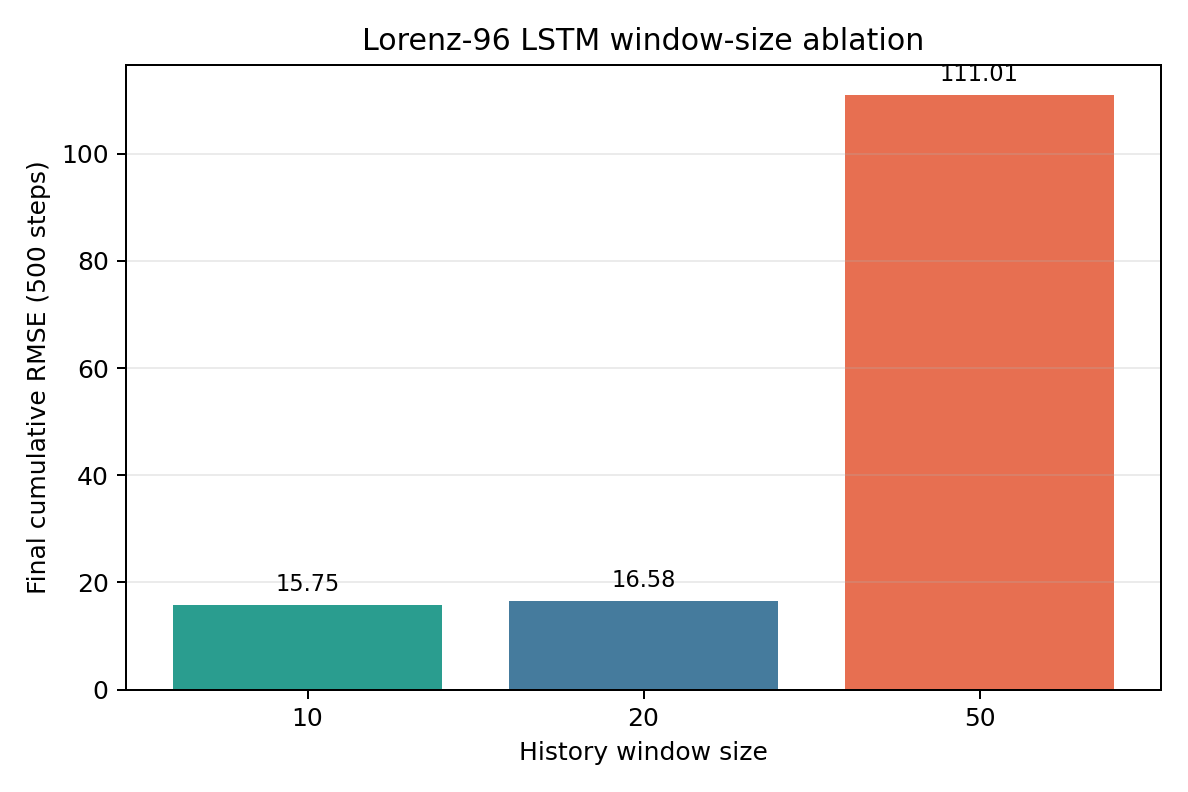
\includegraphics[width=0.62\textwidth]{figures/lorenz96_window_ablation.png}
\caption{Lorenz-96 window-length ablation. The long window $w=50$ severely worsens rollout stability, showing that more history is not always better in chaotic sequences.}
\label{fig:window_ablation_en}
\end{figure}

\subsection{Advanced Architecture Comparison}

Table \ref{tab:advanced_results_en} compares advanced models on the Lorenz-96 500-step rollout task. Baseline LSTM performs worst, with a final cumulative RMSE of 148.79. PINN, Transformer, Refined SS, and Hybrid LSTM all significantly reduce long-term error. Ultimate Hybrid achieves the best result, with a final cumulative RMSE of 12.80.

\begin{table}[htbp]
\centering
\caption{Advanced Lorenz-96 (10D) architecture comparison under 500-step rollout. Data source: \texttt{results/advanced/summary.csv}.}
\label{tab:advanced_results_en}
\begin{tabular}{lc}
\toprule
Model Architecture & Final Cumulative State RMSE \\
\midrule
Baseline LSTM & 148.79 \\
PINN LSTM & 20.18 \\
Refined SS LSTM & 16.79 \\
Transformer & 16.34 \\
Hybrid LSTM & 15.84 \\
\textbf{Ultimate Hybrid} & \textbf{12.80} \\
\bottomrule
\end{tabular}
\end{table}

\begin{figure}[htbp]
\centering
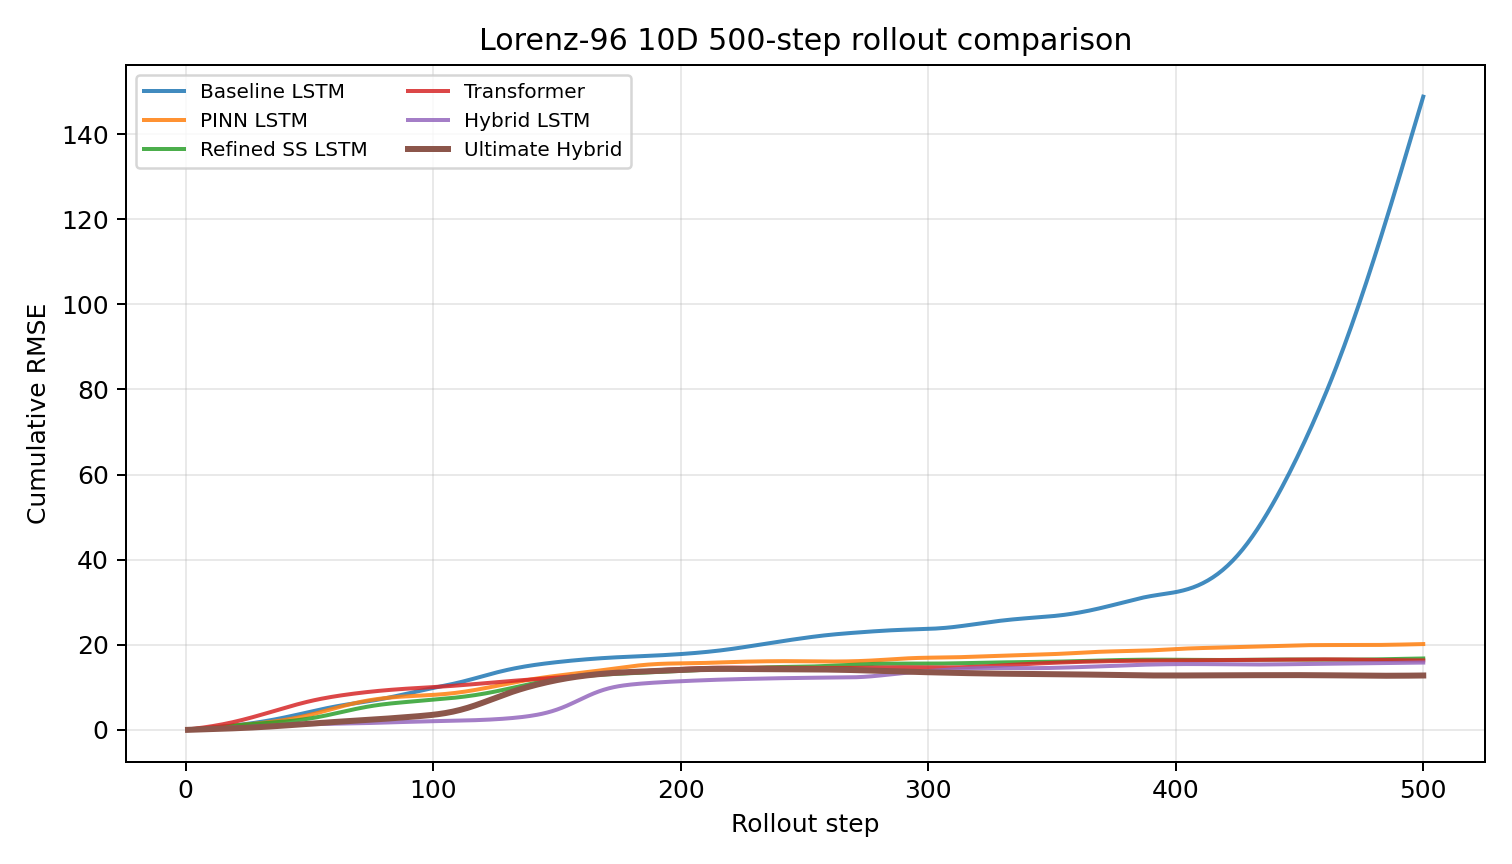
\includegraphics[width=0.86\textwidth]{figures/lorenz96_advanced_rollout_comparison.png}
\caption{Cumulative RMSE curves of advanced Lorenz-96 models under 500-step rollout. Ultimate Hybrid maintains lower error across the test window and achieves the best final RMSE.}
\label{fig:advanced_rollout_en}
\end{figure}

\subsection{Prediction Scatter Analysis}

Following the course requirement for a ``true value vs. predicted value'' scatter plot, Figure \ref{fig:prediction_scatter_en} shows the prediction scatter of Random Forest on the Lorenz-63 short-term task. Most points lie close to the diagonal line, indicating good local short-term fitting. In extreme regions where the absolute value of $x$ is large, the scatter becomes slightly more dispersed, suggesting that highly nonlinear states are more difficult to predict.

This scatter plot mainly reflects one-step or short-horizon fitting quality. It should not be interpreted as evidence of long-term stability. The Lorenz-96 rollout results show that even if the short-term scatter is close to the diagonal, recursive prediction can still diverge due to chaotic sensitivity.

\begin{figure}[htbp]
\centering
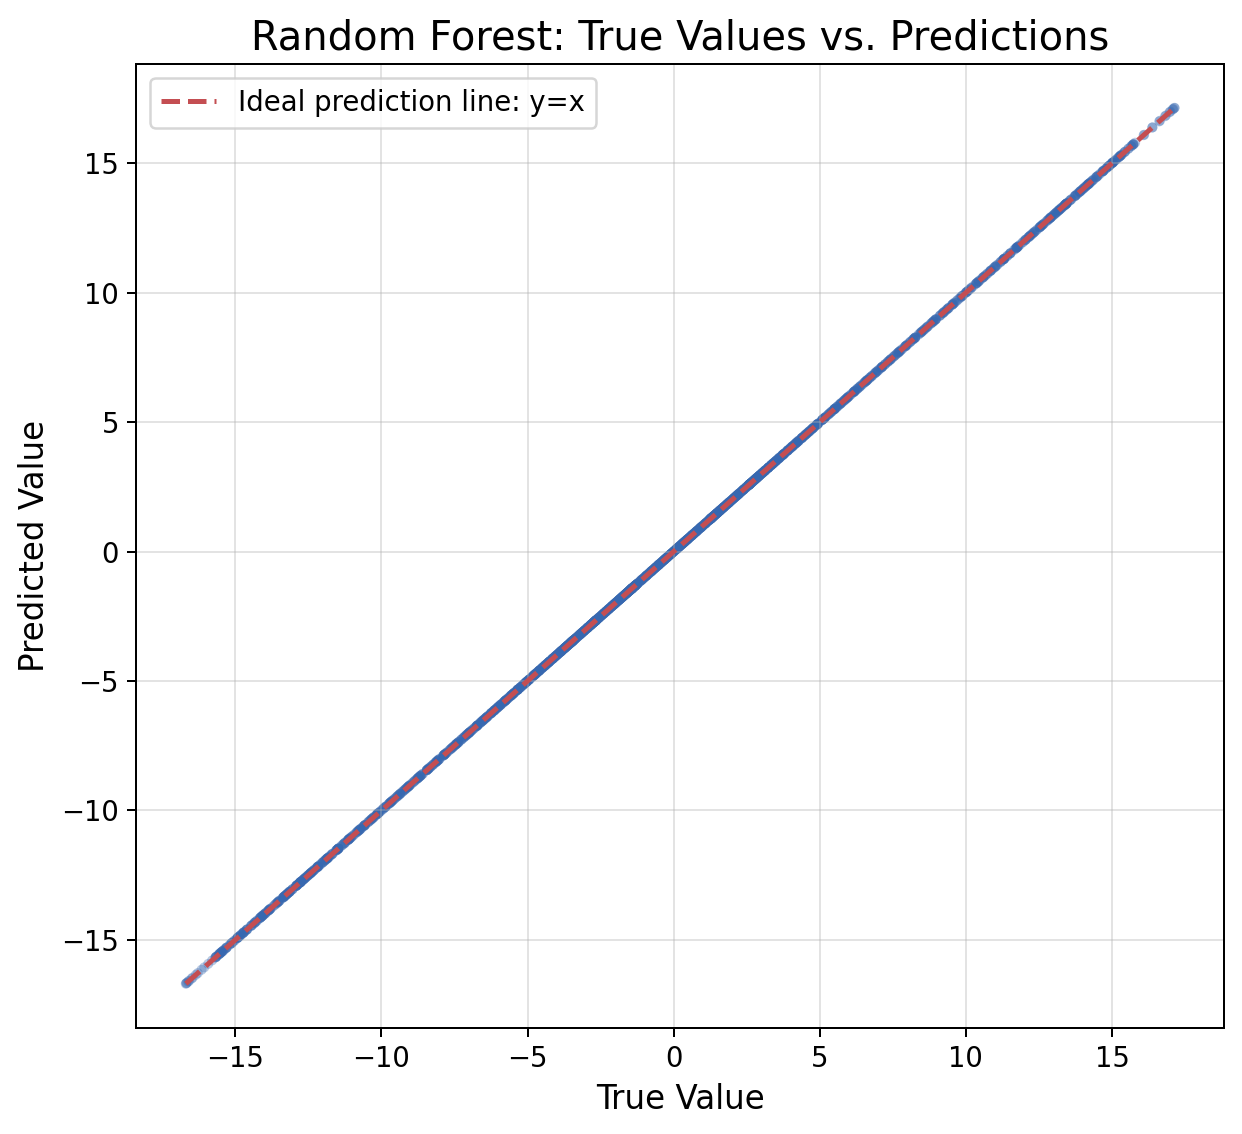
\includegraphics[width=0.62\textwidth]{figures/prediction_scatter_rf_en.png}
\caption{True value vs. predicted value scatter plot for the Lorenz-63 short-term prediction task. Most points are close to the diagonal, but extreme states show larger deviations.}
\label{fig:prediction_scatter_en}
\end{figure}

\subsection{Component Contribution}

PINN LSTM greatly reduces error compared with Baseline LSTM, showing that physical derivative constraints can suppress nonphysical extrapolation. Transformer outperforms Refined SS LSTM, suggesting that self-attention is useful for extracting local evolution patterns from historical windows. Hybrid LSTM further improves the result, showing that even an imperfect physical solver can provide a valuable dynamical basis. Ultimate Hybrid combines these advantages: the physical solver provides a basic evolution direction, Transformer models residuals, PINN constrains update directions, and scheduled sampling brings the training environment closer to rollout.

\subsection{Why One-Step Accuracy Does Not Equal Long-Term Stability}

The results repeatedly show that one-step RMSE and rollout RMSE are not monotonically related. The reasons include:
\begin{enumerate}
    \item one-step evaluation uses true historical windows, while rollout uses predicted historical windows;
    \item high-dimensional chaotic systems amplify small per-step errors;
    \item once predictions leave the neighborhood of the true attractor, later input distributions differ from training data;
    \item a low one-step MSE may reflect local average fitting rather than preservation of dynamical structure.
\end{enumerate}
Therefore, long-horizon rollout stability should be treated as the central evaluation criterion for high-dimensional chaotic prediction.

\section{Discussion}

\subsection{Division of Labor Between Physics and Deep Learning}

The Ultimate Hybrid design reflects a key idea in AI for Science: machine learning does not have to replace physical models; instead, it can cooperate with them. For Lorenz-96, the imperfect RK4 solver already contains the main dynamical structure, while Transformer only needs to learn the residual caused by parameter bias and model error. This decomposition is more stable than learning the entire state transition from data.

\subsection{Limitations of Different Modules}

Residual learning reduces the learning difficulty but does not guarantee long-term stability. Scheduled sampling can reduce train-test mismatch, but an inappropriate schedule may expose the model to noisy predictions too early. PINN loss constrains the update direction but requires a proper loss weight. Transformer improves historical-window modeling but increases training cost. Hybrid physics depends on the physical model being structurally reasonable; if the physical model is seriously wrong, residual learning may also fail.

\subsection{Experimental Limitations}

This project is still limited by the scale of a course assignment. Lorenz-96 is tested only with $N=10$ and $F=8.0$. The number of training epochs is fixed at 20, and large-scale hyperparameter search is not performed. The results mainly come from a single random seed. In future work, more systematic ablation studies could be conducted, such as Transformer + PINN, Transformer + Hybrid, and Hybrid + PINN combinations.

\section{Conclusion}

Starting from Lorenz-63, this paper shows that short-term local state transitions can be learned by supervised models, but long-term recursive rollout is limited by chaotic error amplification. The study then focuses on the 10-dimensional Lorenz-96 system and compares multiple deep-learning architectures under 500-step rollout.

The experiments demonstrate that one-step prediction accuracy is not sufficient to represent long-term prediction ability. Residual LSTM, PINN, Transformer, hybrid physics, and scheduled sampling improve rollout stability from different perspectives. The final Ultimate Hybrid model, which integrates an imperfect physical solver, Transformer residual modeling, PINN loss, and refined scheduled sampling, achieves the lowest final cumulative RMSE of 12.80.

Overall, the main conclusion is that high-dimensional chaotic prediction should not rely only on black-box one-step supervised learning. A more effective route is to use physical models as the dynamical backbone, apply deep learning to residual correction, and improve rollout stability through multi-step training and physical constraints.

\section{Reflection on AI Collaboration}

In this project, LLMs were mainly used for topic decomposition, experimental-route discussion, debugging suggestions, result organization, and report restructuring. They helped us realize that ``good one-step prediction'' is not a sufficient research conclusion, and pushed the project from Lorenz-63 short-term supervised learning to Lorenz-96 long-horizon architecture design.

At the same time, LLM-generated explanations must be verified by code and data. All numerical values in this report come from actual CSV outputs, and the formulas and model descriptions are checked against Python implementations. In this project, LLMs are collaboration tools rather than sources of experimental conclusions.

\appendix

\section{LLM Interaction and Prompt Engineering Log}

\subsection{Problem Definition and Architecture Design}

At the early stage, we asked the LLM the following core question: ``We can already use MLP and Random Forest to make short-term predictions for Lorenz-63, but long-term rollout diverges quickly. Please help us extend this course project into a machine-learning modeling problem that better reflects AI for Science, and suggest a reasonable model comparison route.'' The LLM suggested shifting the evaluation focus from one-step RMSE to recursive rollout and introducing Lorenz-96 as a high-dimensional chaotic system.

Based on this suggestion, we defined the research problem as predicting future Lorenz-96 states from historical windows while maintaining 500-step rollout stability. The LLM also suggested organizing the project around a progression from pure data-driven models to physics-constrained models and finally to physics-residual hybrid models. This became the basis for the Baseline LSTM, PINN LSTM, Transformer, Hybrid LSTM, and Ultimate Hybrid comparison.

\subsection{Core Debugging Record}

A typical debugging case occurred when extending LSTM from one-step training to multi-step scheduled sampling. The original code trained only on true historical windows, while rollout repeatedly appended predicted states back into the window. We sent tensor shapes, window-update code, and error messages to the LLM and asked how to concatenate predicted states into a tensor of shape \texttt{[batch, window, dim]}. The LLM pointed out that the oldest state should be removed along the time dimension and that \texttt{pred.unsqueeze(1)} should be concatenated to the end of the window.

The key lesson was that the LLM did not know our data dimensions unless we explicitly provided context such as \texttt{X.shape}, \texttt{pred.shape}, window length, state dimension, and the full error message. Therefore, later interactions treated LLM code as suggestions to be verified rather than final answers.

\section{Reproducibility}

The main experiment files include:
\begin{itemize}
    \item \texttt{lorenz\_chaos\_prediction.ipynb}: Lorenz-63 supervised learning and hybrid correction;
    \item \texttt{lorenz96\_lstm.py}, \texttt{lorenz96\_lstm\_phase2.py}, and \texttt{lorenz96\_lstm\_phase3.py}: stage-wise Lorenz-96 LSTM optimization;
    \item \texttt{lorenz96\_advanced\_experiments.py}: comparison among PINN, Transformer, Hybrid LSTM, and Ultimate Hybrid.
\end{itemize}
Basic results are saved in \texttt{results/*.csv}, and advanced model results are saved in \texttt{results/advanced/*.csv}. The main comparison table in this report is derived from \texttt{results/advanced/summary.csv}, and rollout curves are generated from the corresponding \texttt{*\_rollout.csv} files.

\begin{thebibliography}{99}

\bibitem{lorenz1963}
Lorenz, E. N. (1963).
Deterministic nonperiodic flow.
\textit{Journal of the Atmospheric Sciences}, 20(2), 130--141.

\bibitem{hochreiter1997}
Hochreiter, S., \& Schmidhuber, J. (1997).
Long short-term memory.
\textit{Neural Computation}, 9(8), 1735--1780.

\bibitem{vaswani2017}
Vaswani, A., Shazeer, N., Parmar, N., Uszkoreit, J., Jones, L., Gomez, A. N., Kaiser, L., \& Polosukhin, I. (2017).
Attention is all you need.
\textit{Advances in Neural Information Processing Systems}.

\bibitem{raissi2019}
Raissi, M., Perdikaris, P., \& Karniadakis, G. E. (2019).
Physics-informed neural networks: A deep learning framework for solving forward and inverse problems involving nonlinear partial differential equations.
\textit{Journal of Computational Physics}, 378, 686--707.

\bibitem{pedregosa2011}
Pedregosa, F., Varoquaux, G., Gramfort, M., Michel, V., Thirion, B., Grisel, O., Blondel, M., Prettenhofer, M., Weiss, R., Dubourg, V., Vanderplas, J., Passos, A., Cournapeau, D., Brucher, M., Perrot, M., \& Duchesnay, E. (2011).
Scikit-learn: Machine learning in Python.
\textit{Journal of Machine Learning Research}, 12, 2825--2830.

\bibitem{virtanen2020}
Virtanen, P., Gommers, R., Oliphant, M., Haberland, M., Reddy, T., Cournapeau, D., Peterson, P., Weckesser, W., Bright, J., van der Walt, S., Brett, M., Wilson, W., Millman, K., Mayorov, N., Nelson, A., Jones, E., Kern, R., Larson, E., Carey, C., Polat, I., Feng, Y., Moore, E., VanderPlas, J., Laxalde, D., Perktold, J., Cimrman, R., Henriksen, I., Quintero, E., Harris, C., Archibald, A., Ribeiro, A., Pedregosa, F., \& van Mulbregt, P. (2020).
SciPy 1.0: Fundamental algorithms for scientific computing in Python.
\textit{Nature Methods}, 17, 261--272.

\end{thebibliography}

\end{document}
